% !TeX encoding = UTF-8
% !TeX spellcheck = pl_PL



% $Id:$

%Author: Wojciech Domski
%Szablon do ząłożeń projektowych, raportu i dokumentacji z steorwników robotów
%Wersja v.1.0.0
%


%% Konfiguracja:
\newcommand{\kurs}{Wizualizacja danych sensorycznych}
\newcommand{\formakursu}{Projekt}

%odkomentuj właściwy typ projektu, a pozostałe zostaw zakomentowane
\newcommand{\doctype}{Za\l{}o\.{z}enia projektowe} %etap I
%\newcommand{\doctype}{Raport} %etap II
%\newcommand{\doctype}{Dokumentacja} %etap III

%wpisz nazwę projektu
\newcommand{\projectname}{Wizualizacja samopozycjonującej się platformy fotowoltanicznej}

%wpisz akronim projektu
%\newcommand{\acronim}{HURA}

%wpisz Imię i nazwisko oraz numer albumu
\newcommand{\osobaA}{Albert \textsc{Lis}, 235534}
%w przypadku projektu jednoosobowego usuń zawartość nowej komendy
%\newcommand{\osobaB}{Micha\l{} \textsc{Moru\'n}, 235986}

%wpisz termin w formie, jak poniżej dzień, parzystość, godzina
\newcommand{\termin}{Śr 17:05 }

%wpisz imię i nazwisko prowadzącego
\newcommand{\prowadzacy}{dr in\.{z}. Bogdan \textsc{Kreczmer}}

\documentclass[10pt, a4paper]{article}
\usepackage[utf8]{inputenc}
\usepackage{polski}
\usepackage[usenames,dvipsnames]{xcolor}

%Preambuła dokumentu

% linki w spisie tresci, bibliografi
\usepackage[bookmarks=true,bookmarksnumbered=false,unicode=true,pdftex=true, colorlinks,filecolor=black,linkcolor=black,urlcolor=black,citecolor=black]{hyperref}

%ustawienie rozmiaru papieru
\usepackage[a4paper, left=2.5cm, right=2.5cm, top=2.5cm, bottom=2.5cm, headsep=1.2cm]{geometry}

%rozmaite ustawienia pozwalające okreslić język

%NALEŻY wybrać jeden z pakietów
%\usepackage{polski} %przydatne podczas składania dokumentów w j. polskim
\usepackage[polish]{babel}  % pakiet lokalizujący dokument w języku polskim
%\usepackage[british]{babel}

\usepackage{indentfirst}	% polski styl pisania (np. rozpoczecie pierwszego akapitu
% pod nazwa rozdzialu od wciecia)
%\usepackage[OT4]{fontenc}
\usepackage[utf8]{inputenc} % w miejsce utf8 można wpisać latin2 bądź cp1250,
% w zależności od tego w jaki sposób kodowane są 
% polskie znaki diakrytyczne przy wprowadzaniu 
% z klawiatury.
%kodowanie znaków, zależne od systemu
\usepackage[T1]{fontenc} %poprawne składanie polskich czcionek

%OPEROWANIE NA OBRAZACH
\usepackage{graphicx}       % pakiet graficzny, umożliwiający m.in.
% import grafik w formacie eps
%\usepackage{epstopdf}		% pozwala na importowanie grafik w formacie eps
% przy użyciu pdflatex
\usepackage[update,prepend]{epstopdf}
\usepackage{rotating}       % pakiet umożliwiający obracanie rysunków
\usepackage{subfigure}      % pakiet umożliwiający tworzenie podrysunków
\usepackage{epic}           % pakiet umożliwiający rysowanie w środowisku latex
\usepackage{psfrag}         % pakiet umożliwiający podmianę łańcuchów znaków 
% w plikach eps
%\usepackage{curves}         % pakiet do wykreslania krzywych

%pakiety dodające dużo dodatkowych poleceń matematycznych
\usepackage{amsfonts}       % pakiet z rozmaitymi czcionkami matematycznymi
%\usepackage{amssymb}        % pakiet z rozmaitymi symbolami matematycznymi
\usepackage{amsmath}        % pakiet z rozmaitymi środowiskami matematycznymi

\usepackage{fp}             % pakiet z funkcjami operujacymi 
% na liczbach zmiennoprzecinkowych
\usepackage{calc}           % pakiet umożliwiający operacje arytmetyczne
% na tzw. licznikach (liczbach całkowitych)
\usepackage{leftidx}		% indeksy górne i dolne po lewej stronie

%definicje matematyczne
\providecommand{\abs}[1]{\lvert#1\rvert}
\providecommand{\norm}[1]{\lVert#1\rVert}

%pakiety wspomagające i poprawiające składanie tabel
\usepackage{supertabular}
\usepackage{array}
\usepackage{tabularx}
\usepackage{hhline}
\usepackage{longtable}		% wsparcie dla dlugich tabel
\usepackage{multicol}		% podzial strony na wiele kolumn

%pakiet do BibTex
\usepackage{cite}

\usepackage{url} %pakiet pozawalający na dodawanie adresów url w bibliografi

%pakiet wypisujący na marginesie etykiety równań i rysunków zdefiniowanych przez \label{}, chcąc wygenerować finalną wersję dokumentu wystarczy usunąć poniższą linię
%\usepackage{showlabels}

\usepackage{float}			% lepsza obsluga mechanizmow obiektow plywajacych
% wymuszenie wstawienia np. tabeli, obrazka w danym miejscu przez [H]

\usepackage{listings}       % pakiet dedykowany zrodlom programow
\usepackage{color}


\definecolor{dkgreen}{rgb}{0,0.6,0}
\definecolor{gray}{rgb}{0.5,0.5,0.5}
\definecolor{mauve}{rgb}{0.58,0,0.82}

\lstset{ %
	language=C,                % the language of the code
	basicstyle=\small,           % the size of the fonts that are used for the code
	numbers=left,                   % where to put the line-numbers
	numberstyle=\footnotesize\color{gray},  % the style that is used for the line-numbers
	stepnumber=1,                   % the step between two line-numbers. If it's 1, each line 
	% will be numbered
	numbersep=5pt,                  % how far the line-numbers are from the code
	backgroundcolor=\color{white},      % choose the background color. You must add \usepackage{color}
	showspaces=false,               % show spaces adding particular underscores
	showstringspaces=false,         % underline spaces within strings
	showtabs=false,                 % show tabs within strings adding particular underscores
	%frame=single,                   % adds a frame around the code
	rulecolor=\color{black},        % if not set, the frame-color may be changed on line-breaks within not-black text (e.g. comments (green here))
	tabsize=2,                      % sets default tabsize to 2 spaces
	captionpos=b,                   % sets the caption-position to bottom
	breaklines=true,                % sets automatic line breaking
	breakatwhitespace=false,        % sets if automatic breaks should only happen at whitespace
	%title=\lstname,                   % show the filename of files included with \lstinputlisting;
	% also try caption instead of title
	keywordstyle=\color{blue},          % keyword style
	commentstyle=\color{dkgreen},       % comment style
	stringstyle=\color{mauve},         % string literal style
	escapeinside={\%*}{*)},            % if you want to add LaTeX within your code
	morekeywords={*,...},              % if you want to add more keywords to the set
	deletekeywords={...}              % if you want to delete keywords from the given language
}

%polish signs in lst code
\lstset{literate=%
	{ą}{{\k{a}}}1
	{ć}{{\'c}}1
	{ę}{{\k{e}}}1
	{ł}{{\l}}1
	{ń}{{\'n}}1
	{ó}{{\'o}}1
	{ś}{{\'s}}1
	{ż}{{\.z}}1
	{ź}{{\'z}}1
	{Ą}{{\k{A}}}1
	{Ć}{{\'C}}1
	{Ę}{{\k{E}}}1
	{Ł}{{\L}}1
	{Ń}{{\'N}}1
	{Ó}{{\'O}}1
	{Ś}{{\'S}}1
	{Ż}{{\.Z}}1
	{Ź}{{\'Z}}1
}

\usepackage{verbatim}       % pakiet dedykowany rozmaitym wydrukom tekstowym
\usepackage{ifthen}         % pakiet umożliwiający tworzenie prostych programów
% (m.in. zawiera instrukcje powtórzeniowe 
% i warunkowe)
\usepackage{upquote}		%normal quotations marks ' and `

% deklaracje wymagane przez pakiet theorem automatycznie ladowany w przypadku
% klasy dokumentu article
%
\newtheorem{Dn}{Definicja}[section]     % deklaracja srodowiska definicja
\newtheorem{La}[Dn]{Lemat}                % deklaracja srodowiska lemat
\newtheorem{Tm}[Dn]{Twierdzenie}          % deklaracja srodowiska twierdzenie
\newtheorem{Rk}[Dn]{Spostrze{\.z}enie}  % deklaracja srodowiska spostrzezenie
\newtheorem{Am}[Dn]{Algorytm}           % deklaracja srodowiska algorytm
\newtheorem{As}[Dn]{Za{\l}o{\.z}enie}   % deklaracja srodowiska zalozenie
\newtheorem{Pn}[Dn]{Propozycja}           % deklaracja srodowiska propozycja
\newtheorem{Py}[Dn]{W{\l}asno{\'s}{\'c}}  % deklaracja srodowiska wlasnosc
\newtheorem{Cy}[Dn]{Wniosek}              % deklaracja srodowiska wniosek
\newtheorem{Ee}[Dn]{Przyk{\l}ad}        % deklaracja srodowiska przyklad
\newtheorem{Ex}{{\'C}wiczenie}          % deklaracja srodowiska cwiczenie

%helps to specify width of a column in table
%\begin{tabular}{|C{1cm}|c|c|c|c|c|c|c|c|c|c|}
%first column will have widht of 1cm
\newcolumntype{L}[1]{>{\raggedright\let\newline\\\arraybackslash\hspace{0pt}}m{#1}}
\newcolumntype{C}[1]{>{\centering\let\newline\\\arraybackslash\hspace{0pt}}m{#1}}
\newcolumntype{R}[1]{>{\raggedleft\let\newline\\\arraybackslash\hspace{0pt}}m{#1}}

\sloppy			%zawija bardzo długie linie

%\pagenumbering{gobble}% Remove page numbers (and reset to 1)
	
\begin{document}

\def\tablename{Tabela}	%zmienienie nazwy tabel z Tablica na Tabela

\begin{titlepage}
	\begin{center}
		\textsc{\LARGE \formakursu}\\[1cm]		
		\textsc{\Large \kurs}\\[0.5cm]		
		\rule{\textwidth}{0.08cm}\\[0.4cm]
		{\huge \bfseries \doctype}\\[1cm]
		{\huge \bfseries \projectname}\\[0.5cm]
%		{\huge \bfseries \acronim}\\[0.4cm]
		\rule{\textwidth}{0.08cm}\\[1cm]
		
		\begin{flushright} \large
	%	\emph{Skład grupy:}\\
		\osobaA\\[0.4cm]
	%	\osobaB\\[0.4cm]
		
		\emph{Termin: }\termin\\[0.4cm]

		\emph{Prowadzący:} \\
		\prowadzacy \\
		
		\end{flushright}
		
		\vfill
		
		{\large \today}
	\end{center}	
\end{titlepage}

\newpage
\tableofcontents
\newpage

\section{Opis projektu}
\label{sec:OpisProjektu}

Celem projektu jest stworzenie wizualizacji 3D platformy fotowoltanicznej. Platforma jest sterowana za pomocą mikrokontrolera i czterech czujników. Dzięki temu ma możliwość podążania za najintensywniejszym źródłem światła i pozycjonowania się w sposób umożliwiający optymalne korzystanie z energii słonecznej. Dane o pozycji platformy zostaną przesłane do komputera PC. W komputerze zostanie uruchomiona aplikacja pozwalająca pokazywać aktualną pozycję platformy.
\newline
\newline

\begin{figure}[H]
	\centering
	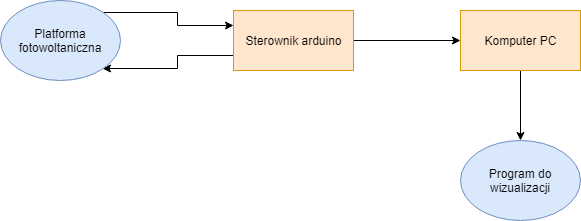
\includegraphics[width=1\textwidth]{figures/diag_uml.png}
	\caption{Architektura systemu}
	\label{fig:Architektura}
\end{figure}

\section{Założenia projektowe}

	\subsection{Komunikacja}
	\begin{enumerate}
		\item Połączenie ze sterownikiem
		\newline
		Realizowane za pomocą modułu Wi-Fi ESP8266 i protokołu UDP/TCP lub bez łączności bezprzewodowej z użyciem portu szeregowego.
		\item Połączenie modułu Wi-Fi z mikrokontrolerem
		\newline
		Realizowane za pomocą portu szeregowego.
	\end{enumerate}

	\subsection{Wizualizacja}
	\begin{enumerate}
		\item Środowisko
		\newline
		Zostanie wykorzystany silnik graficzny UNITY w darmowej wersji.
		\item Modele
		\newline
		Zostaną wygenerowane za pomocą programu Blender.
		\item Tekstury
		\newline
		Zostaną stworzone za pomocą programu GIMP lub pobrane z dowolnej internetowej bazy z darmowymi teksturami.
	\end{enumerate}

\newpage
%Obecne w dokumencie do etapu I
\section{Harmonogram pracy}

	\subsection{Zakres prac}
		\begin{enumerate}
			\item Zapoznanie się ze środowiskiem UNITY
			\newline
			Stworzenie kilku prostych projektów tak aby zapoznać się ze środowiskiem i jego możliwościami.
			
			\item Stworzenie podstawowego modelu 3D
			\newline
			Stworzenie prostego modelu platformy bez dbałości o detale.
			
			\item Implementacja obrotów platformy za pomocą klawiatury
			\newline
			Stworzenie wizualizacji poruszania się modelu za pomocą strzałek na klawiaturze.
			
			\item Stworzenie dokładnych modeli w programie Blender
			\newline
			Stworzenie dokładnego odwzorowania platformy z uwzględnieniem połączeń krawędzi.
			
			\item Wygenerowanie tekstur
			\newline
			Stworzenie lub pobranie z internetu tekstur dla obiektów.
			
			\item Opracowanie standardu komunikacji sterownik - PC
			\newline
			Zastanowienie się nad sposobem przesyłania informacji oraz ich kodowaniem.
			
			\item Implementacja komunikacji sterownik - PC
			\newline
			Implementacja jednostronnej komunikacji między sterownikiem a PC.
			
			\item Implementacja obrotów platformy za pomocą danych ze sterownika
			\newline
			Modyfikacja istniejącego sterowania w taki sposób aby zwizualizowany stan platformy zgadzał się z rzeczywistym.
			
			\item Poprawki stylistyczne
			\newline
			Poprawa elementów które okazały się niedopracowane w trakcie projektu.
		\end{enumerate}
	
	\subsection{Kamienie milowe}
		\begin{enumerate}
			\item Implementacja działającej wizualizacji w oparciu o sterowanie klawiaturą
			\item Implementacja poprawnej komunikacji sterownik - PC
			\item Implementacja wizualizacji w oparciu o dane ze sterownika
		\end{enumerate}
	
	\subsection{Wykres Gantta}
	
	\begin{figure}[H]
		\centering
		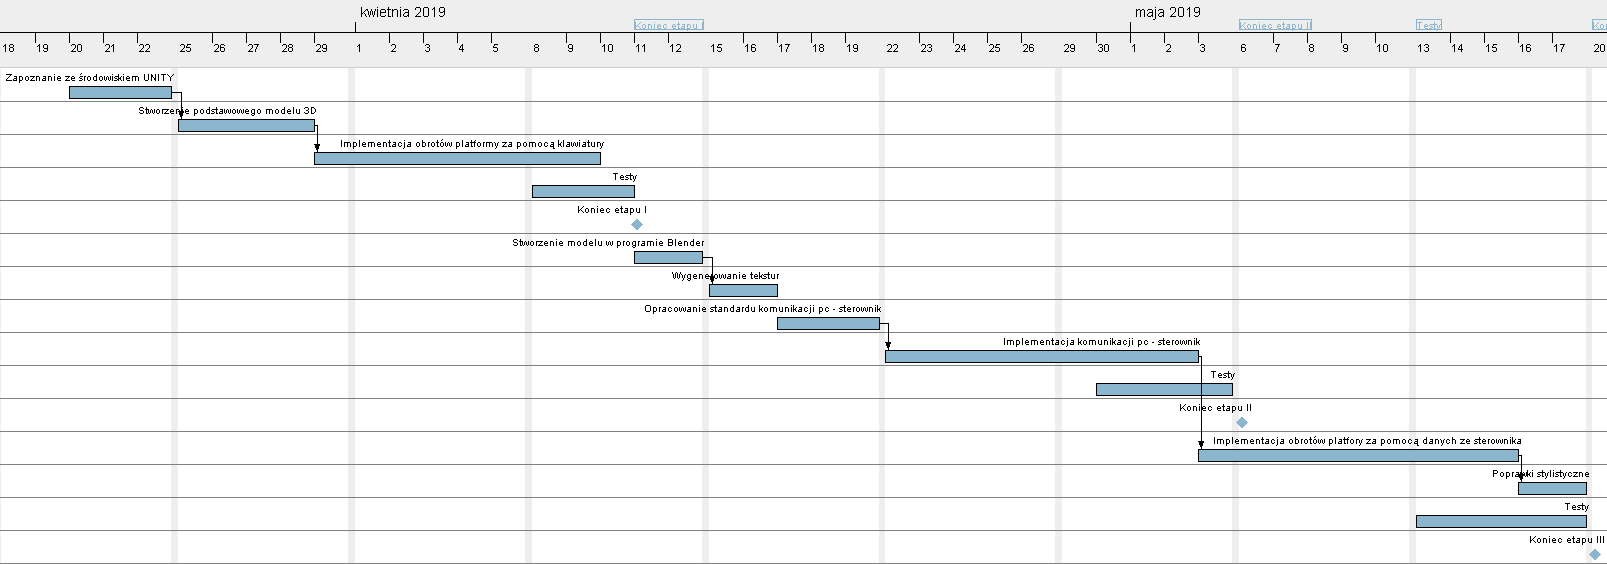
\includegraphics[width=1.4\textwidth, angle = 90]{figures/harm1.png}
		\caption{Diagram Gantta}
		\label{fig:DiagramGantta}
	\end{figure}

\section{Projekt interfejsu graficznego}
	\subsection{Funkcjonalność UI}
		\begin{enumerate}
			\item Lista wyboru nazwy portu szeregowego
				\newline
				Powinna umożliwić wybranie portu do którego podłączony jest sterownik.
			\item Lista wyboru prędkości połączenia
				\newline
				Powinna zawierać takie prędkości wyrażone w bodach względem których przesłanie pakietu danych będzie trwało mniej niż 1/60[s]. 
			\item Przycisk nawiązania połączenia
				\newline
				Przycisk umożliwiający nawiązanie połączenia ze sterownikiem po wybraniu odpowiednich parametrów.
			\item Przycisk zakończenia połączenia
				\newline
				Przycisk umożliwiający zakończenie połączenia ze sterownikiem.
			\item Przycisk zamknięcia aplikacji
				\newline
				Przycisk umożliwiający zamknięcie aplikacji. Powinien realizować również akcję zamykania połączenia jeśli nadal by było ono otwarte.	
		\end{enumerate}
	
	\subsection{Funkcjonalność aplikacji}
		\begin{enumerate}
			\item Wyświetlanie aktualnej wartości natężenia światła
				\newline	
				Wartość natężenia światła powinna być wyświetlana nad platformą np w postaci napisu 3D.
			\item Wyświetlanie aktualnej pozycji
				\newline	
				Powyżej/poniżej wartości natężenia światła powinna być wyświetlana informacja o aktualnej pozycji. Za pomocą schematu XYZ.
		\end{enumerate}
	
	\subsection{Graficzna reprezentacja aplikacji}
		\begin{enumerate}[I.]
			\item Schemat
				\begin{figure}[H]
					\centering
					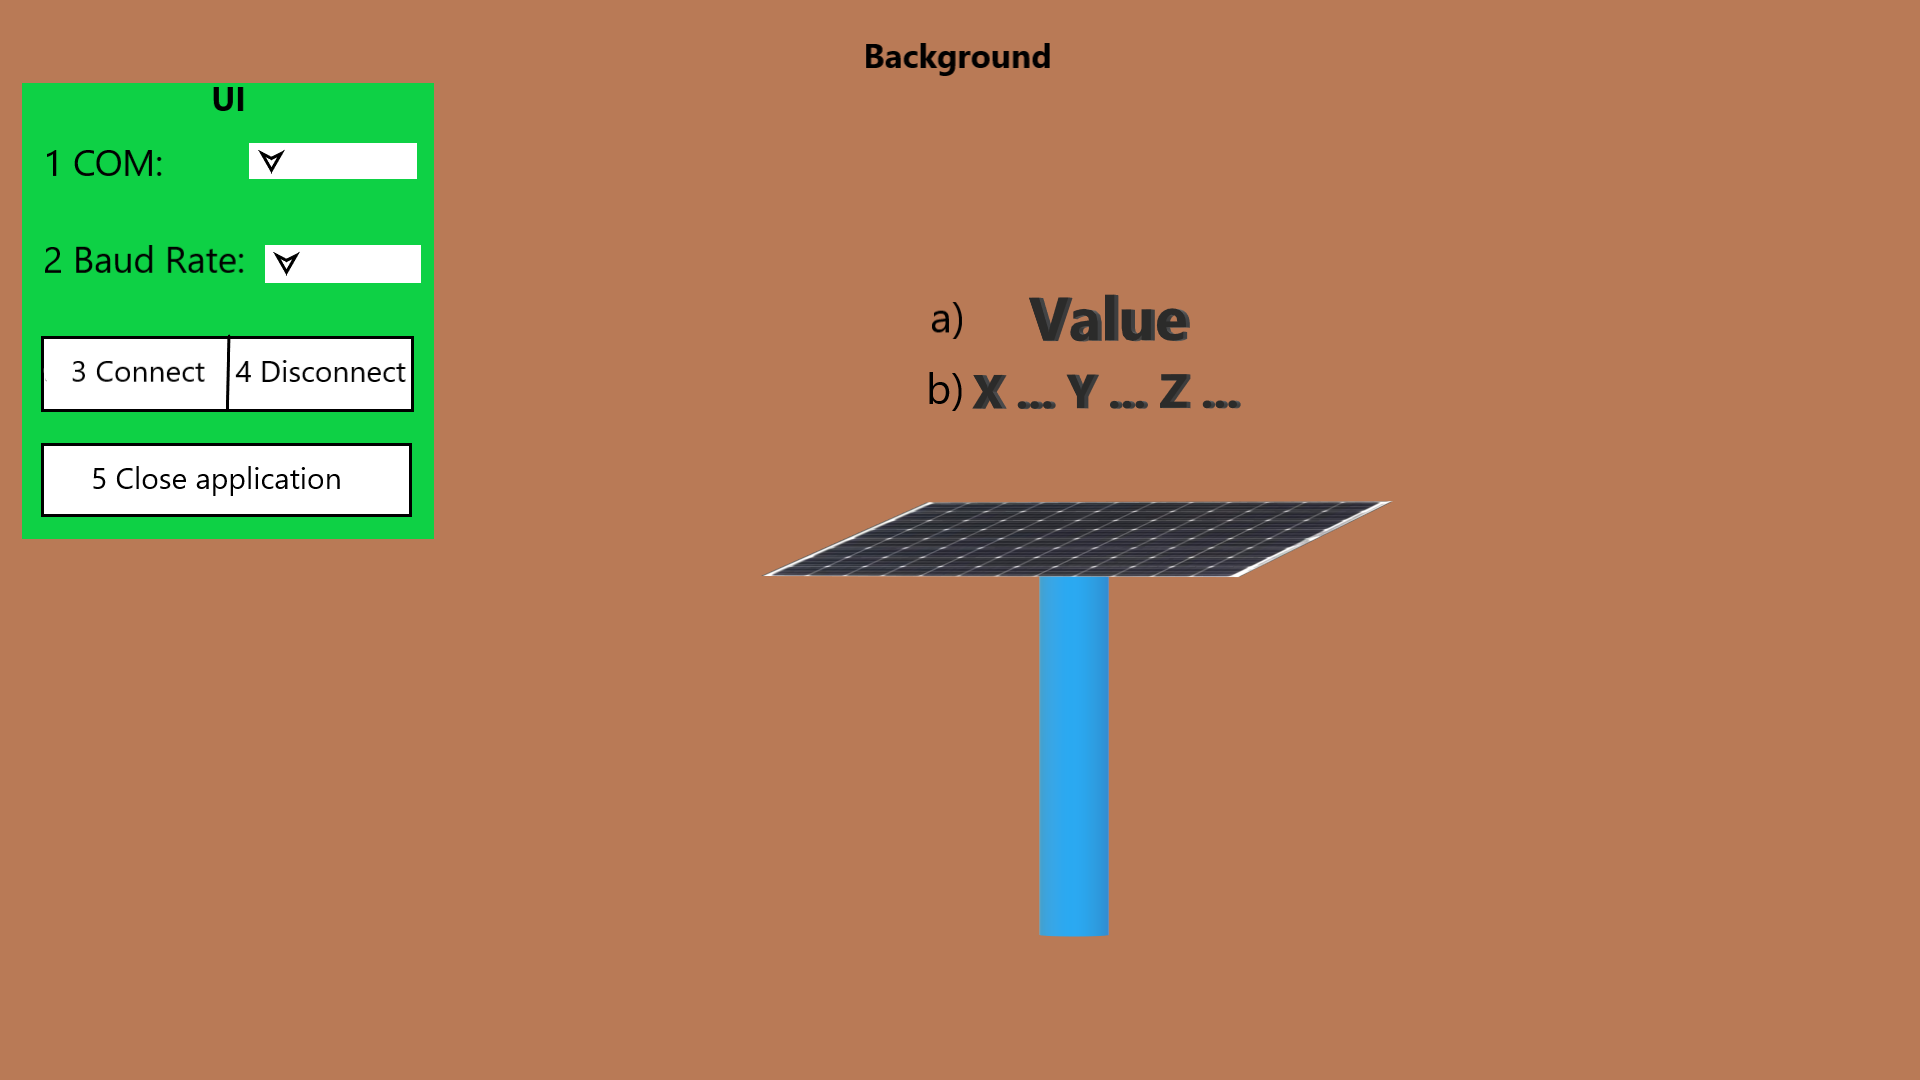
\includegraphics[width=1\textwidth]{figures/paint.png}
					\caption{Wygląd aplikacji}
					\label{fig:ArchitekturaBD1}
				\end{figure}
			\newpage
			\item Szczegółowy opis UI
				\begin{enumerate}[1]
					\item COM
						\newline	
						Lista modyfikująca parametr odpowiedzialny za nazwę portu w skrypcie obsługi portu szeregowego.
					
					\item Baud Rate
						\newline	
						Lista modyfikująca parametr odpowiedzialny za prędkość transmisji w skrypcie obsługi portu szeregowego.
					
					\item Connect
						\newline	
						Przycisk wywołujący funkcję odpowiedzialną za nawiązanie połączenia w skrypcie obsługi portu szeregowego.
						
					\item Disconnect
						\newline	
						Przycisk wywołujący funkcję odpowiedzialną za zamknięcie połączenia w skrypcie obsługi portu szeregowego.
						
					\item Close application
						\newline	
						Przycisk wywołujący skrypt odpowiedzialny za zamknięcie aplikacji.
				\end{enumerate}
			\item Szczegółowy opis napisów interaktywnych
			\begin{enumerate}[a)]
				\item Value
				\newline	
				Napis wyświetlający bieżącą wartość natężenia światła. Połączony ze skryptem rotacji aby dostosowywał swoje położenie względem kamery.
				
				\item X \dots Y \dots Z \dots
				\newline	
				Napis wyświetlający aktualne położenie we współrzędnych kartezjańskich. Połączony ze skryptem rotacji aby dostosowywał swoje położenie względem kamery.
			\end{enumerate}
		\end{enumerate}
			
\newpage
\section{Wstępne rezultaty}
		\subsection{Zmiany w projekcie}
		Nastąpiła zmiana środowiska programistycznego z Unity na Qt + OpenGL. To pociągnęło za sobą zmiany w harmonogramie pracy i podejście do projektu. Najpierw zostanie stworzona komunikacja między PC a sterownikiem a następnie wizualizacja 3D. Dodatkowo zmieni się format przesyłanych danych. Aktualnie przewiduję że pakiet danych będzie wyglądał następująco: 
		\begin{center}
			"H\footnote{rotacja horyzontalna} ... V\footnote{rotacja wertykalna} ... L\footnote{natężenie światła} ... I\footnote{Zmierzone natężenie prądu} ... CRC\footnote{32-bitowa suma kontrolna} ... $\backslash$n\footnote{znak końca pakietu danych}".
		\end{center}
		Gdzie ... to poszczególne wartości. Natomiast separator to znak spacji.
		
		\subsection{Zrealizowane zadania}
			\begin{enumerate}
				\item \textbf{Graficzy interfejs użytkownika} \newline
				Stworzyłem aplikację komunikującą się ze sterownikiem za pomocą portu szeregowego. Aplikacja po uruchomieniu prosi o podanie prędkości komunikacji w bodach oraz portu do którego został przyłączony sterownik. Domyślna prędkość to 9600 bodów. Natomiast lista portów wczytuje tylko te dostępne.
				\begin{figure}[H]
					\centering
					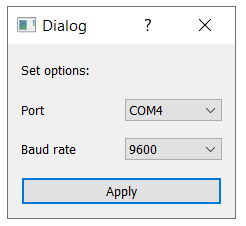
\includegraphics[width=0.3\textwidth]{figures/opcje.png}
					\caption{Okno opcji}
					\label{fig:opcje}
				\end{figure}
				
				Po zaakceptowaniu ustawień uruchamia się okno główne w którym mamy opcje Connect oraz Disconnect. Obie wzajemnie się wykluczają. Dodatkowo gdy połączenie jest aktywne wygaszona zostaje opcja zmiany ustawień połączenia.
				
				\begin{figure}[H]
					\centering
					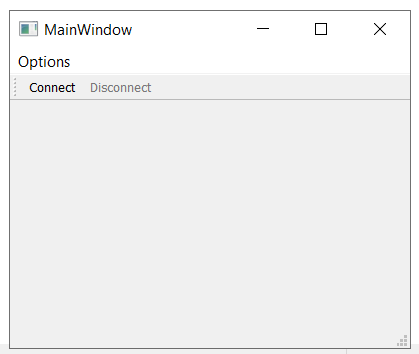
\includegraphics[width=0.4\textwidth]{figures/okno_glowne.png}
					\caption{Okno główne}
					\label{fig:okno_glowne}
				\end{figure}
			
				\item \textbf{Komunikacja} \newline
				Komunikacja jest uruchamiana w osobnym wątku tak aby nie zakłócać pracy głównego okna. Port szeregowy został skonfigurowany z 8 bitami danych, bitem parzystości oraz bitem stopu. Aktualnie przesyłane dane wyświetlam za pomocą konsoli. Gdy suma kontrolna się nie zgadza wyświetlam komunikat o niepoprawnej ramce danych.
			\end{enumerate}
		
\section{Zaawansowane rezultaty}
	\subsection{Komunikacja}
	Zmianie uległ format danych. Zostały dodane dodatkowe pola. Oraz liczona jest suma kontrolna 8-bitowa. Nazwa sumy: CRC-8-Dallas/Maxim, Wielomian: 0x8C.
		\begin{center}
			"H\footnote{rotacja horyzontalna}... V\footnote{rotacja wertykalna}... L\footnote{natężenie światła}... U\footnote{Napięcie}... I\footnote{Prąd}... P\footnote{Moc}... CRC\footnote{8-bitowa suma kontrolna}... $\backslash$r$\backslash$n\footnote{znak końca pakietu danych}".
		\end{center}
	Przykładowe wyniki:
		\begin{figure}[H]
			\centering
			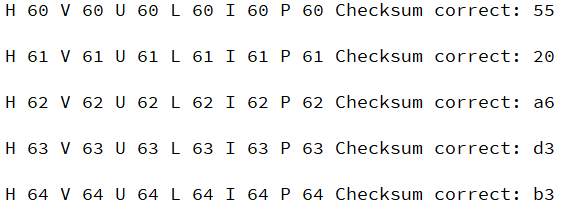
\includegraphics[width=0.6\textwidth]{figures/serial_wyniki.png}
			\caption{Przykładowe wyniki}
			\label{fig:serial_wyniki}
		\end{figure}
	
	\subsection{Graficzny interfejs użytkownika}
		\begin{enumerate}
			\item Okno główne
				\begin{figure}[H]
					\centering
					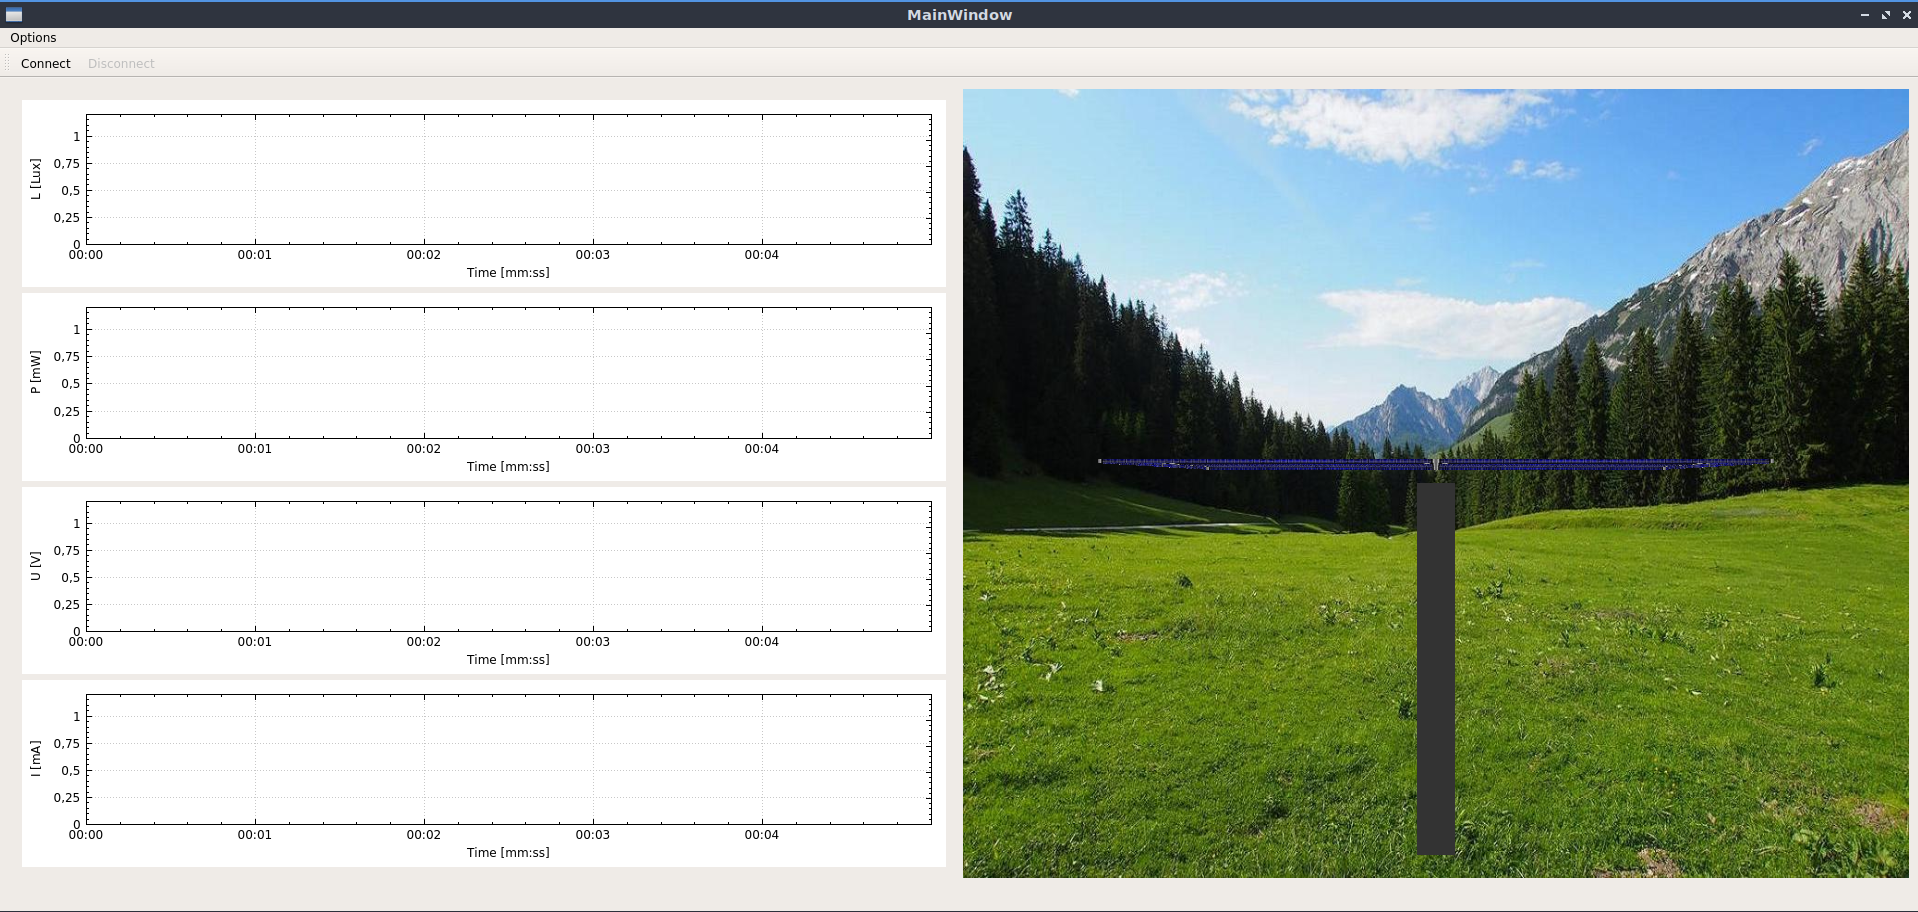
\includegraphics[width=0.98\textwidth]{figures/okno_glowne1.png}
					\caption{Okno główne}
					\label{fig:okno_glowne1}
				\end{figure}
			Po lewej znajdują się wykresy wartości pomiarowych. Natomiast po prawej stronie mamy wizualizację platformy fotowoltaicznej.
					
			\item Wykresy
				\begin{figure}[H]
					\centering
					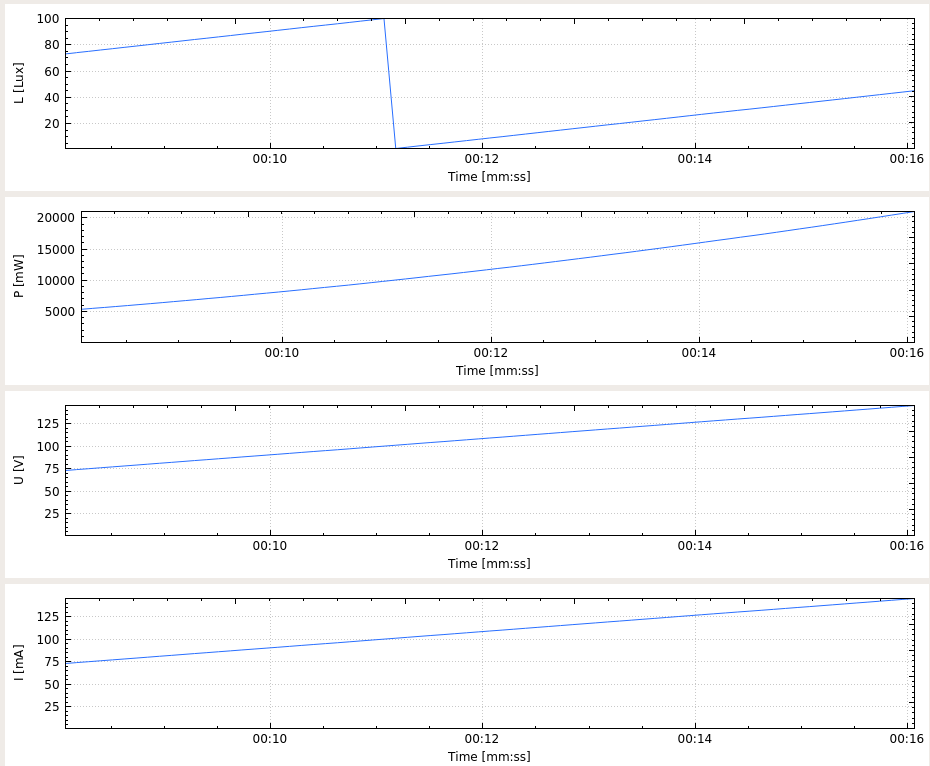
\includegraphics[width=1.0\textwidth]{figures/wykresy.png}
					\caption{Wykresy}
					\label{fig:wykresy}
				\end{figure}
			Do rysowania wykresów używam biblioteki zewnętrznej QCustomPlot. Na osi pionowej znajdują się poszczególne wartości pomiarów. Na osi poziomej mamy czas w formacie minuty:sekundy. Wykres jest dynamiczny o stałym oknie czasowym. Na przykładowym rysunku \ref{fig:wykresy} wynosi ono 8 sekund.
			
			\item Wizualizacja
				\begin{figure}[H]
					\centering
					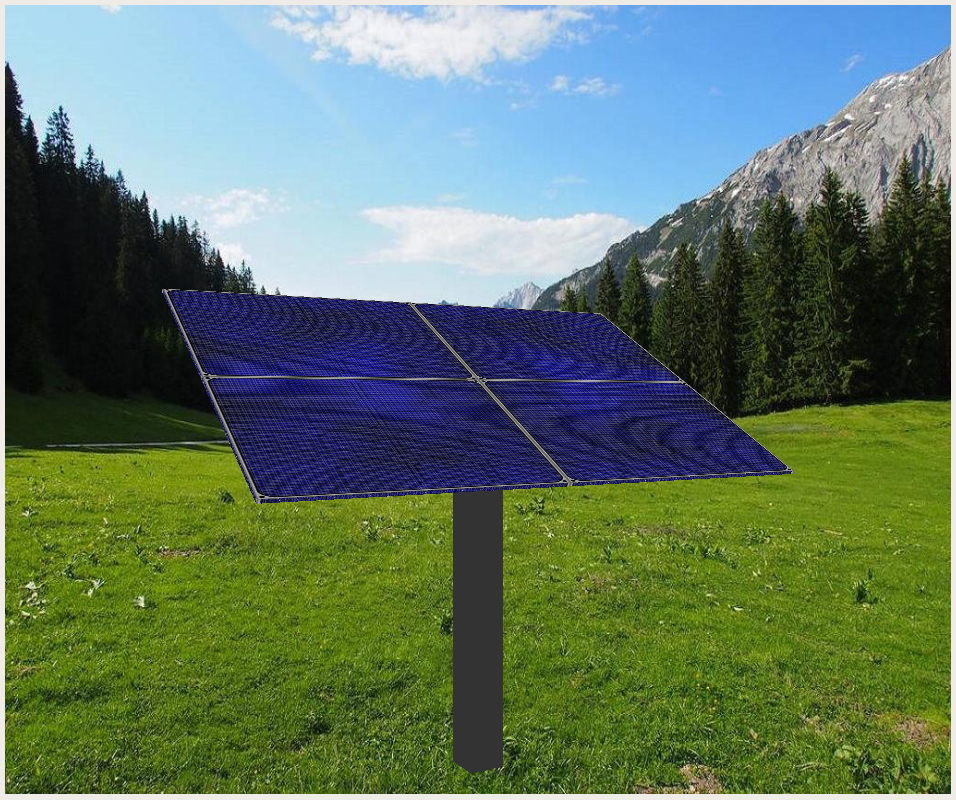
\includegraphics[width=1.0\textwidth]{figures/wizualizacja.png}
					\caption{Wizualizacja}
					\label{fig:wizualizacja}
				\end{figure}
			Zaimplementowałem dwuosiową rotację. Horyzontalna (cała platforma) oraz wertykalna (tylko panel fotowoltaiczny).
		\end{enumerate}
\end{document}







































